%\chapter{Experimentos e Resultados}
\chapter{Experiments and Results}

%\section{O Projeto \textbf{machado}}
\section{The Project \textbf{machado}}

%\par
%Algumas informa��es sobre o aplicativo (linguagem, n�mero de linhas, op��es de execu��o (--help), %\par
%Mostrar gr�fico de ortogonalidade? (m�trica x acur�cia)
%\par
%Mostrar tabela de acertos?
%\par
%O algoritmo n�o ortogonal est� quase igual ao lazy - talvez ele nem precise ser citado
%\par

The project \textbf{machado} contains the implementation of an association rules based classifier with three different approaches.
\par
The first one, called \textbf{non-orthogonal} just obtains the frequent patterns set and generates rules with it. After that, it chooses the more indicated class according to the rules contained in a rank considering confidence.
\par
The second one, called \textbf{orthogonal} obtains an orthogonal set of patterns from the frequent patterns set, and generates rules from that patterns set. After that, it chooses the more indiated class the same way it is done with the non-orthogonal approach.
\par
the third one, called \textbf{ORIGAMI} is an implementation of ORIGAMI, as it was proposed in \cite{zaki07origami}.
\par
The execution options are shown below:

\begin{verbatim}
Usage: ./classifier [options]
Options:
  -i, --training-file        Set the training file
  -t, --testing-file         Set the testing file
  -s, --support              Set the support
  -c, --confidence           Set the confidence
  -r, --run-mode             Set the run mode [c,o] [CLASSICAL, ORTHOGONAL]
  -p, --pattern-set          Set the pattern set type [f,m,r] [FREQUENT, MAXIMAL,
                               RANDOM MAXIMAL]
  -n, --min-num-rules        Set the minimum number of rules
  -l, --max-num-rank-rules   Set the maximum number of rules considered in rank
                               (rank size)
  -m, --min-rule-len         Set the minimum length of the rules
  -x, --max-rule-len         Set the maximum length of the rules
  -o, --orth-mode            Set the orthogonality mode [h,p,o] [HEURISTICAL,
                               POLYNOMIAL, ORIGAMI]
  -e, --orth-metric          Set the orthogonality mode [s,c,l,a] [SIMILARITY,
                               TRANSACTION COVERAGE, CLASS COVERAGE, ALL]
  -w  --orth-method          Set the way metrics are used [s,p,a] [SET, PAIR AVERAGE,
                               ALL]
  -g  --orth-pat-ordering    Set the way patterns are ordered for orthogonality
                              heuristic [s,r,i,z,n] [SORTED, REVERSE SORTED,
                              SORTED BY SIZE, REVERSE SORTED BY SIZE, NONE]
  -a  --origami-alpha        Set the alpha parameter used by ORIGAMI
  -b  --origami-beta         Set the beta parameter used by ORIGAMI
  -d, --debug                Set the level of debug [0-4] [NODEBUG - MAXLEVEL]
  -v, --verbose              Use verbose mode
  -h, --help                 Display this information
\end{verbatim}

Now, we will show some graphics comparing the executions of the three approaches implemented in machado and LAC, the lazy associative classifier impelemted in \cite{Veloso06Lazy}, but first we will do some observations about these test instances:
\par
\begin{itemize}
	\item LAC was run with support 1, just because this is the objective of LAC (the Adriano Veloso implementation) - to get better results with the minimum support value;
	\item ORIGAMI was run with $\alpha = 0.2$, and $\beta = 0.8$, we need to make more tests with another values for $\alpha$ and $\beta$ in order to get better results;
	\item We are still running these experiments with anoter parameters, and trying to get some better results for all approaches.
\end{itemize}
\par
The figure \ref{fig:histogram_acc} shows a histogram with the best accuracies for each dataset obtained with LAC, ORIGAMI, orthogonal classifier and non-orthogonal classifier. The figure \ref{fig:histogram_pat} shows a histogram with the average number of patterns used for each classification, and the figure \ref{fig:histogram_rul} shows the average number of rules generated for each classification. For these three results it was used the best sets of parameters for each application and dataset, for example, considering the orthogonal classifier, for anneal.ac we used support equals to 0.0001, but for waveform.ac we used support equals to 0.01, since the best results were obtained with this value.

\begin{figure}[htbp]
	\centering
	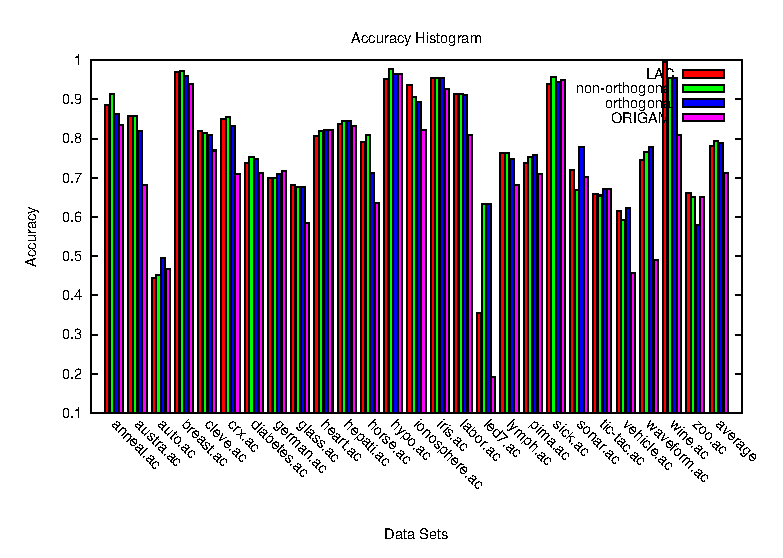
\includegraphics{graphs/histogram_acc.eps}
	\caption{Accuracy Histogram (best results for each dataset)}
	\label{fig:histogram_acc}
\end{figure}

As we can see in the figure \ref{fig:histogram_acc}, the results for accuracy orthogonal and non-orthogonal versions of our classifier are very close. the average accuracy obtained for them were $0.8085$ and $0.8088$ respectively, and they are both better than LAC.

\begin{figure}[htbp]
	\centering
	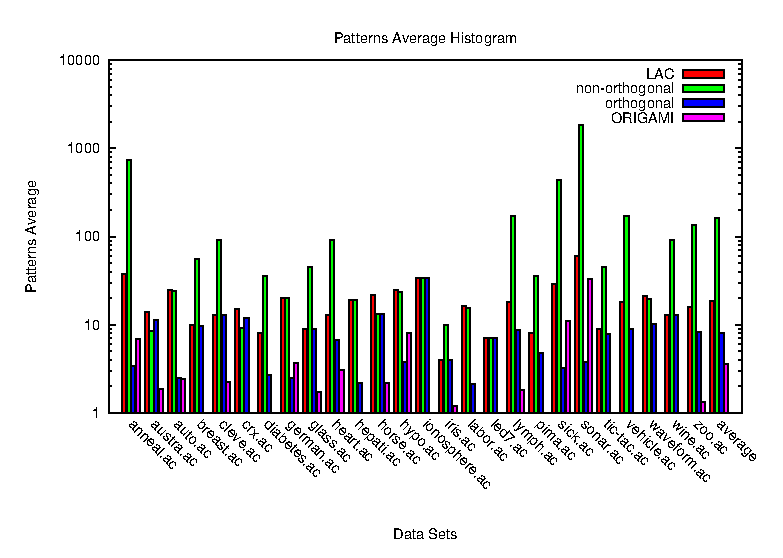
\includegraphics{graphs/histogram_pat.eps}
	\caption{Patterns Histogram (best results for each dataset)}
	\label{fig:histogram_pat}
\end{figure}

The number of patterns generated by orthogonal version of our classifier (shown by figure \ref{fig:histogram_pat}) is lower than the LAC ones. The difference would be still greater (as it was comparing our orthogonal and non-orthogonal versions) if we used lower values for confidence in LAC (the value for this parameter that produced better results in average was $0.95$.

\begin{figure}[htbp]
	\centering
	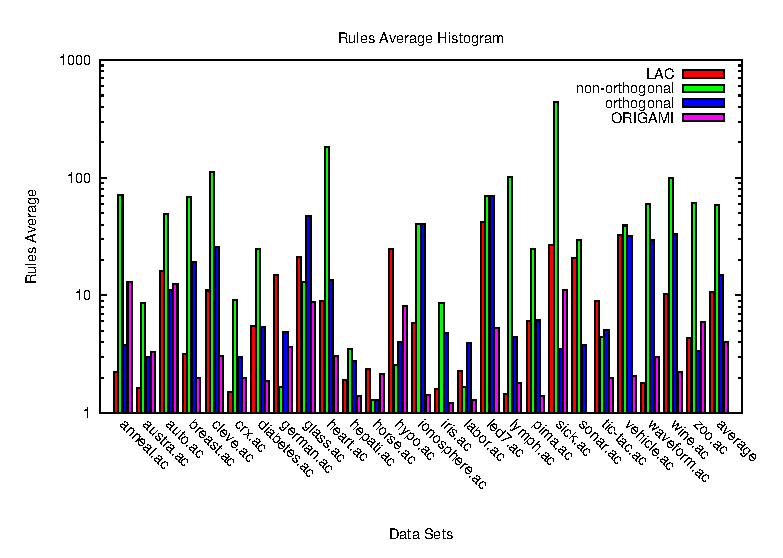
\includegraphics{graphs/histogram_rul.eps}
	\caption{Rules Histogram (best results for each dataset)}
	\label{fig:histogram_rul}
\end{figure}

The number of patterns generated by orthogonal version of our classifier (shown by figure \ref{fig:histogram_rul}) is higher than the LAC ones. This happened because the same - the values for confidence used for LAC were very high. We believe that if we run LAC with lower values for confidence, this number will be much higher.

\clearpage

The figure \ref{fig:bst_histogram_acc} shows a histogram with the best accuracies for each dataset obtained with LAC, ORIGAMI, orthogonal classifier and non-orthogonal classifier. The figure \ref{fig:bst_histogram_pat} shows a histogram with the average number of patterns used for each classification, and the figure \ref{fig:bst_histogram_rul} shows the average number of rules generated for each classification. For those three results it was used, for each application, the set of parameters that produced the best average accuracy for the whole set of data. The values for each parameter are shown in table \ref{tab:parms}.
\par
Some observations about the parameters - the support used by LAC is the absolute value 1 (one transaction), and not a relative value as in the other applications. Some parameters are not applicable to all approaches.

\begin{table}[htbp]
	\centering
		\begin{tabular}{|l|l|l|l|l|}
		\hline
		& \textbf{LAC}	& \textbf{non-orthogonal}	& \textbf{orthogonal} &	\textbf{ORIGAMI}	\\
		\hline
		support		& 1	& 0.0001		& 0.01		& 0.001		\\
		\hline
		confidence	& 0.95	& 0.0001		& 0.001		& 0.1		\\
		\hline
		min-num-rules	& 1	& 1			& 1		& 1		\\
		\hline
	max-num-rank-rules	& 10	& 1000			& 100		& 100		\\
		\hline
		min-rule-len	& 1	& 1			& 1		& -		\\
		\hline
		max-rule-len	& 1	& 1			& 2		& -		\\
		\hline
		metric		& -	& -			& similarity	& similarity	\\
		\hline
		method		& -	& -			& set		& -		\\
		\hline
		pat-ordering	& -	& -			& sorted	& -		\\
		\hline
		alpha		& -	& -			& -		& 0.2		\\
		\hline
		beta		& -	& -			& -		& 0.8		\\
		\hline
		\end{tabular}
	\caption{Set of parameters for each run}
	\label{tab:parms}
\end{table}

\begin{figure}[htbp]
	\centering
	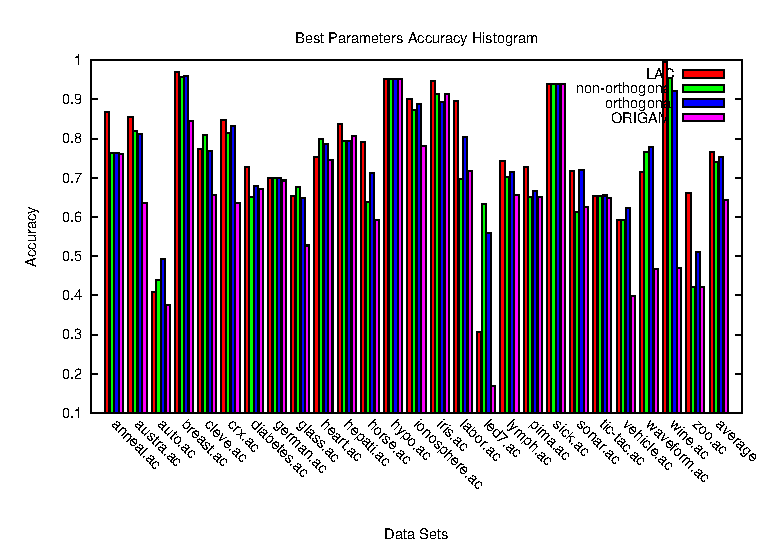
\includegraphics{graphs/bst_histogram_acc.eps}
	\caption{Accuracy Histogram (best average results for all datasets)}
	\label{fig:bst_histogram_acc}
\end{figure}

\begin{figure}[htbp]
	\centering
	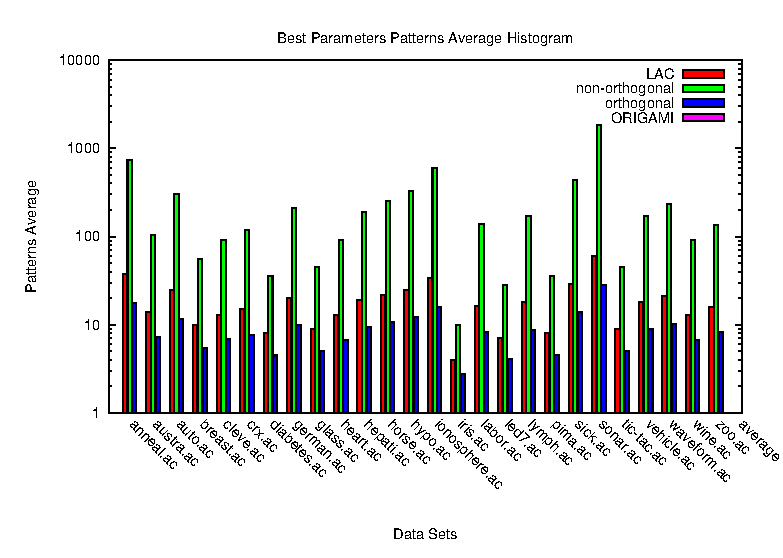
\includegraphics{graphs/bst_histogram_pat.eps}
	\caption{Patterns Histogram (best average results for all datasets)}
	\label{fig:bst_histogram_pat}
\end{figure}

The number of patterns generated with ORIGAMI approach in figure \ref{fig:bst_histogram_pat} was $1$ (one) for all datasets. This happened because the best combined values for support and confidence found was $0.001$ and $0.1$, and this, possibly, didn't generate any valid rule, since the low support generates big maximal patterns, and $0.1$ is a sufficient value for confidence to turn all rules invalid. Since the applicative tries to generate, at least, one rule for each test instance, just one of the rules is added to the result. As it was told before, we are running the experiment with more parameter combinations, searching for better results.

\begin{figure}[htbp]
	\centering
	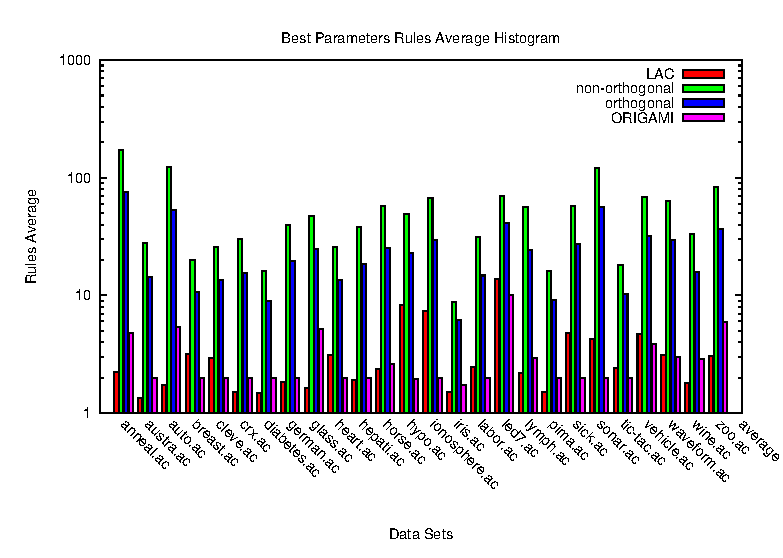
\includegraphics{graphs/bst_histogram_rul.eps}
	\caption{Rules Histogram (best average results for all datasets)}
	\label{fig:bst_histogram_rul}
\end{figure}

\clearpage

\section{Compara��o Ortogonal x N�o Ortogonal}

Histogramas de acur�cia, n�mero de padr�es e n�mero de regras. \\
Comparar melhor conjunto de par�metros para cada arquivo e melhor conjunto de par�metros para todos os arquivos juntos.

\section{Compara��o Ortogonal x LAC}

Histogramas de acur�cia, n�mero de padr�es e n�mero de regras. \\
Comparar melhor conjunto de par�metros para cada arquivo e melhor conjunto de par�metros para todos os arquivos juntos.

\section{Compara��o Ortogonal x ORIGAMI}

Histogramas de acur�cia, n�mero de padr�es e n�mero de regras. \\
Comparar melhor conjunto de par�metros para cada arquivo e melhor conjunto de par�metros para todos os arquivos juntos.
